% This is the master file of the folder structure. In order to compile your document, run this file. In most LaTeX editors, the master file can be specified such that the document can also be compiled from the other .tex files (in the docs folder).

% First, the preamble needs to be called. This contains all the 'under the hood' stuff for your document.
% This file contains your LaTeX preamble. A preamble is a part of your document where all required packages and macros can be defined. This needs to be done before the \begin{document} command.

% Documentclass:
% Standard LaTeX classes are: article, book, report, slides, and letter. These cover the basis, but are not best. More advanced users might want to try out the KOMA classes or the memoir class. Optional arguments: 10pt. The font size of the main content is set to 10pt with the option between [].
\documentclass[10pt]{report}

% Geometry:
% The papersize of the document is defined with the geometry package. Here, the size is set to A4 with a4paper. Other possibilities are a5paper, b5paper, letterpaper, legalpaper and executivepaper.
\usepackage[a4paper]{geometry}

% AMS math packages:
% Required for proper math display.
\usepackage{amsmath,amsfonts,amsthm}

% Graphicx:
% If you want to include graphics in your document, the graphicx package is required.
\usepackage{graphicx}

% Booktabs:
% The booktabs package is needed for better looking tables. 
\usepackage{booktabs}

% SIunitx:
% The SIunitx package enables the \SI{}{} command. It provides an easy way of working with (SI) units.
\usepackage{siunitx}

% URL:
% Clickable URL's can be made with this package: \url{}.
\usepackage{url}

% Caption:
% For better looking captions. See caption documentation on how to change the format of the captions.
\usepackage{caption}

% Hyperref:
% This package makes all references within your document clickable. By default, these references will become boxed and colored. This is turned back to normal with the \hypersetup command below.
\usepackage{hyperref}
	\hypersetup{colorlinks=false,pdfborder=0 0 0}

% Cleveref:
% This package automatically detects the type of reference (equation, table, etc.) when the \cref{} command is used. It then adds a word in front of the reference, i.e. Fig. in front of a reference to a figure. With the \crefname{}{}{} command, these words may be changed.
\usepackage{cleveref}
	\crefname{equation}{equation}{equations}
	\crefname{figure}{figure}{figures}	
	\crefname{table}{table}{tables}

% The title page is created with the command \maketitle which needs to be placed after the \begin{document} command. To create the titlepage, some entries are needed: the name of the autor is defined by \author{}, the title by the entry \title{} and the date by the command \date{}. Note that the current date is displayed with \today.
\author{First von Last}
\title{Title of document}
\date{\today}

% All the actual content of your document should be placed after \begin{document} and before \end{document}. This content should be placed in the docs folder and can then be called with \input{docs/filename}.
\begin{document}

% Here the actual title page is printed, based on the given entries \author{}, \title{} and \date{}.
\maketitle

% The table of contents can be automatically generated with the \tableofcontents command. Note that you need to compile the document twice in order to see the changes in the table of contents.
\tableofcontents

% The \input{} command reads and processes the indicated example.tex file. Note that docs/ locates the folder where the .tex file is stored.
% A chapter named 'Your first document' is created
\chapter{Your first document} \label{cha:your-first-document}


% A section called 'Basics' is created
\section{Basics} \label{sec:basics}

Text is formatted with: \textbf{bold}, \textit{italic} and \underline{underline}.
\Cref{sec:basics} is part of \cref{cha:your-first-document}.


% A subsection named 'Typesetting content' is created
\section{Typesetting content} \label{sec:typesetting}


% A subsubsection named 'Equations' is created
\subsection{Equations} \label{subsec:equations}

% Inline equations
An example of an inline equation is: the derivative of $x^2$ is $2x$. \Cref{eq:example} shows a display equation:
% Display equations
\begin{align} \label{eq:example}
          y_{0} &= \frac{\sqrt{256}}{2} \\
                &= 2^{3} = 8 \nonumber 
\end{align}


\subsection{Units} \label{subsec:units}

% % Working with units
An easy way to work with (SI) units: \SI{1}{\hertz} is equal to \SI{2\pi}{\radian\per\second}.


\subsection{Figures} \label{subsec:figures}

% Inserting a figure
Here a figure named \textit{logo.pdf} is inserted\footnote{The \textit{logo.pdf} file is located in the figs folder.}:
\begin{figure}[h]
  \centering
  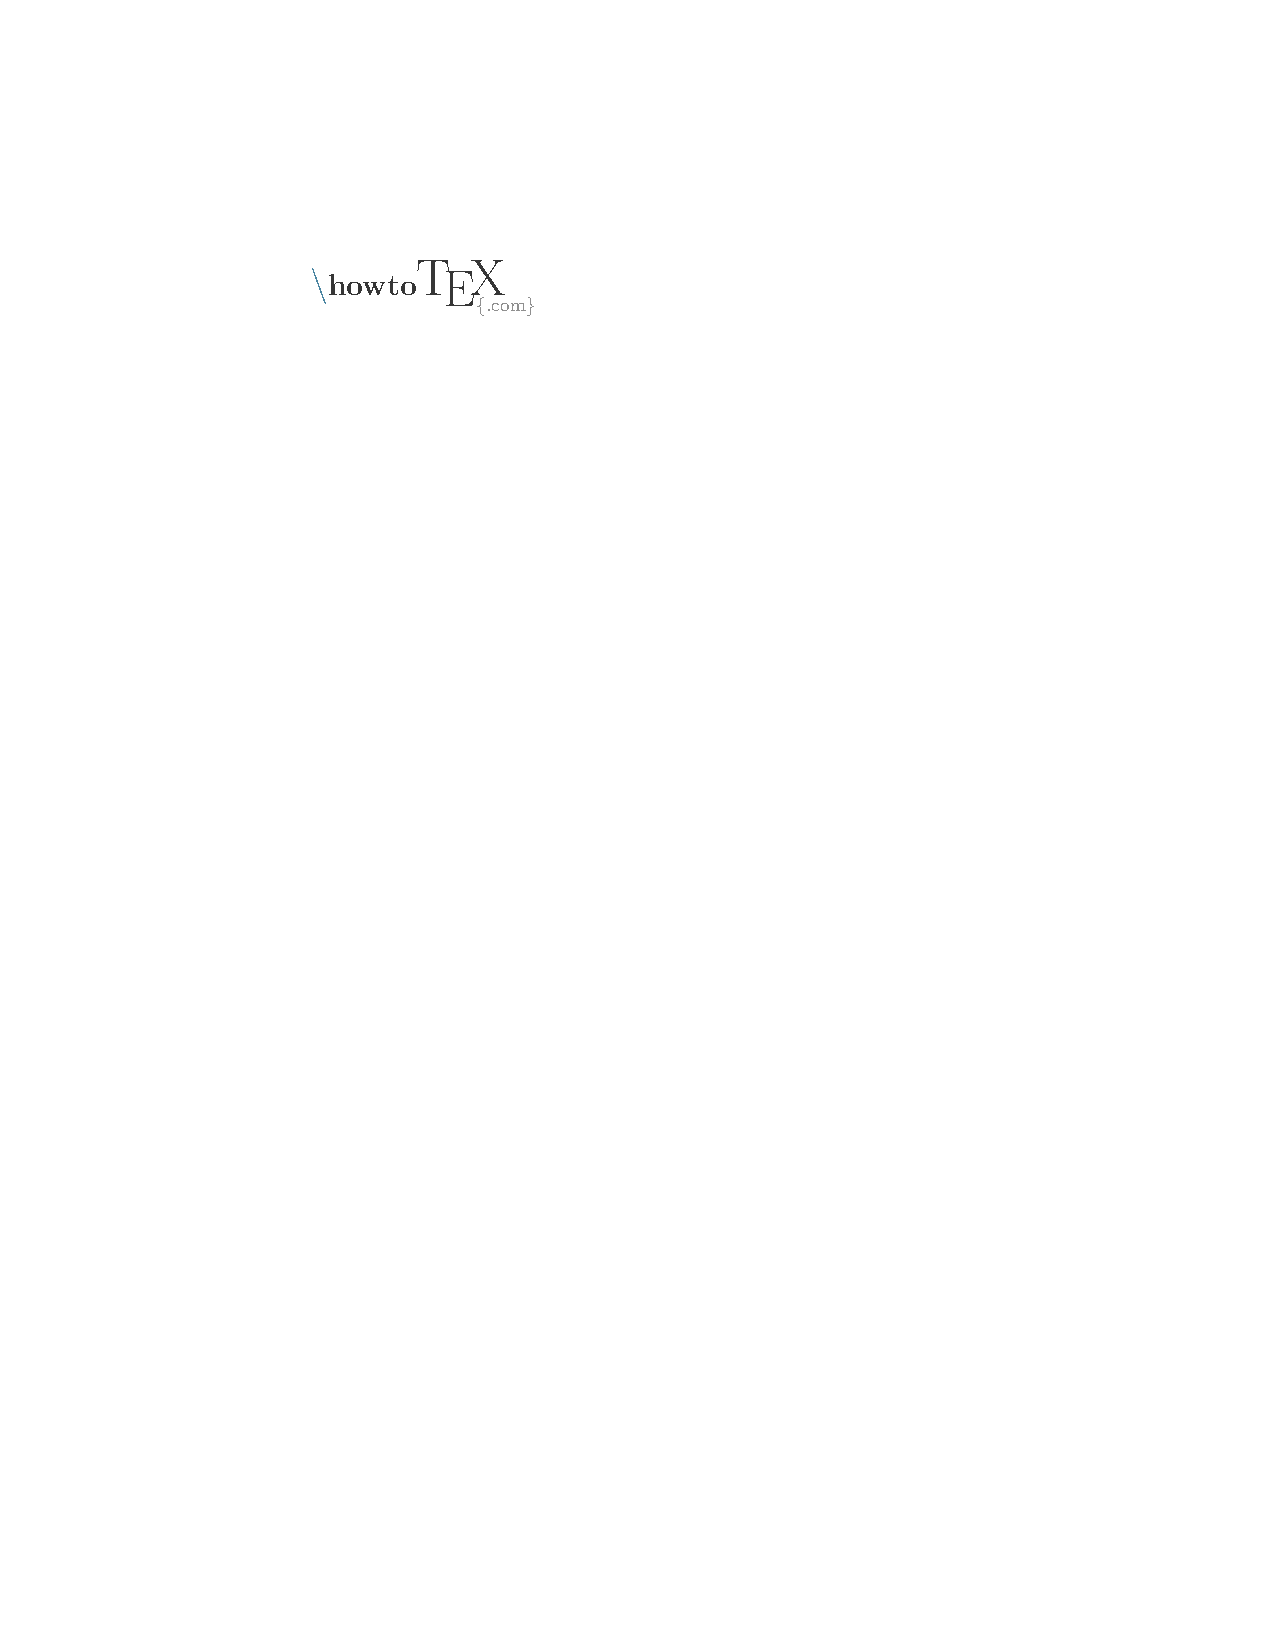
\includegraphics[width=50mm]{figs/logo}
  \caption{Caption example}
  \label{fig:logo}
\end{figure}


\subsection{Tables} \label{subsec:tables}

% Inserting a table
A table is shown in \cref{tb:table}.
\begin{table}[h]
  \centering
  \caption{Caption example}
  \label{tb:table}
  \begin{tabular}{crl}
    \toprule
    Name     & Grade & Year    \\
    \midrule
    John     & 7.5   & 2012\\
    Richard  & 2     & 2010\\
    \bottomrule
  \end{tabular}
\end{table}


\subsection{Lists} \label{subsec:lists}
% Creating lists
%% Here a subsubsection is created. Note that this section is not shown in the table of content.
\subsubsection{Numbered}
Creating a numbered list:
\begin{enumerate}
  \item First entry
  \item Second entry
\end{enumerate}

\subsubsection{Descriptive}
Creating a descriptive list:
\begin{description}
  \item[First] entry
  \item[Second] entry
\end{description}


\section{Reference to bibliography items} \label{sec:bibliography}
First are reference to a website is made \cite{MiscEntry}, then a reference to an article \cite{ArticleEntry} and finally a reference to a book \cite{last2012}.

\paragraph{Good luck!}

% The bibliography is printed with \bibliography{}. With the command \bibliographystyle{} a style is picked.
\bibliographystyle{plain}
\bibliography{refs/references}

% To close your document, add the \end{document} command. Everything after this command will not be processed.
\end{document}